
\section{Getting started}\label{sect:start}\index{PISM!getting started}

In this section we give an extended example applying PISM to the Greenland ice sheet.  We use recent data sets provided by the Sea-level Response to Ice Sheet Evolution (\href{http://websrv.cs.umt.edu/isis/index.php/SeaRISE_Assessment}{SeaRISE}), a community-organized process to produce an upper bound of ice sheet contributions to sea level in the next 100--200 years.

The example in this section is a quick, hands-on first look at PISM.  It is not an in-depth tutorial, and many details of what is happening will only be explained later.  The sections on the older EISMINT-Greenland and EISMINT-Ross modeling cases, for instance, do a more complete job of explaining the ways users will need to preprocess not-so-clean input data and then make, and evaluate, modeling choices.

The PISM output figures in this section were produced using a supercomputer.  However, in order for the examples here to run on a typical workstation, a rather coarse $20\,\textrm{km}$ grid is used.  The purpose of PISM is to make much higher spatial resolution actually possible, but it requires large-scale \emph{parallel} processing.


\subsection{Install PISM}

See the \emph{Installation Manual}
   \begin{center}
     \href{http://www.pism-docs.org/dev/pdfs/installation-dev.pdf}{\t{www.pism-docs.org/dev/pdfs/installation-dev.pdf}}
   \end{center}
to install PISM.  Once installed, an executable \verb|pismr|, and several others, will be in the \verb|bin| subdirectory of the main PISM directory.  The main PISM directory might be at \verb|/home/username/pism-dev/|, for example.  The instructions below assume you start from that main PISM directory.  We also assume you are using a \verb|bash| shell or at least one that accepts \verb|bash| syntax.


\subsection{Obtain and preprocess the input data}

The NetCDF data file which we use for input is freely-available at, and is described by, this web page: 
\medskip

\centerline{\protect{\textbf{\url{http://websrv.cs.umt.edu/isis/index.php/Present_Day_Greenland}}}}
\medskip

\noindent The quickest way to get the file itself is to do

\verb|$ cd examples/searise-greenland|

\verb|$ ./preprocess.sh|

\noindent The script \verb|preprocess.sh|\footnote{\protect{This script requires \texttt{wget} and NCO (NetCDF Operators; \url{http://nco.sourceforge.net/})}.} downloads the ``master'' present-day data set and adjusts it to make it PISM-readable.\footnote{The script looks for \texttt{Greenland\_5km\_v0.93.nc}.  If a different version number is desired, edit the script to change the line ``\texttt{DATAVERSION=0.93}''.}

Preprocessing creates three NetCDF files from the master data, each of which has small ``metadata'' changes so that they can be read by PISM.  The metadata itself can be listed at the command line, or put in a text file, by \verb|ncdump -h|.  Two of the new files contain famous time-dependent paleo-climate records from ice core (GRIP; \verb|pism_dT.nc|) and seabed core records (SPECMAP; \verb|pism_dSL.nc|).

Any of these NetCDF files can be viewed with \verb|ncview| or other NetCDF visualization tools.  (See Table \ref{tab:NetCDFview} below.)  Application of \verb|pyNGL| tools to \verb|Greenland_5km_v0.93.nc| produced figures \ref{fig:sr-input1} and  \ref{fig:sr-input1}, for example.

\begin{figure}[ht]
\centering
\mbox{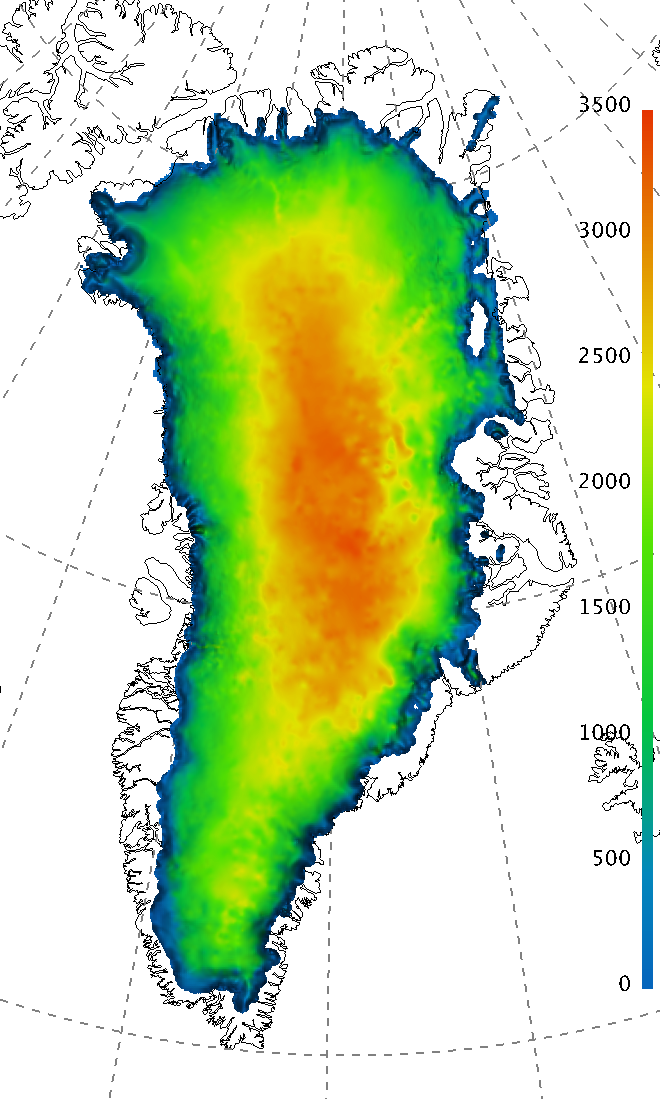
\includegraphics[width=2.5in,keepaspectratio=true]{sr-greenland-thk}
 \qquad\qquad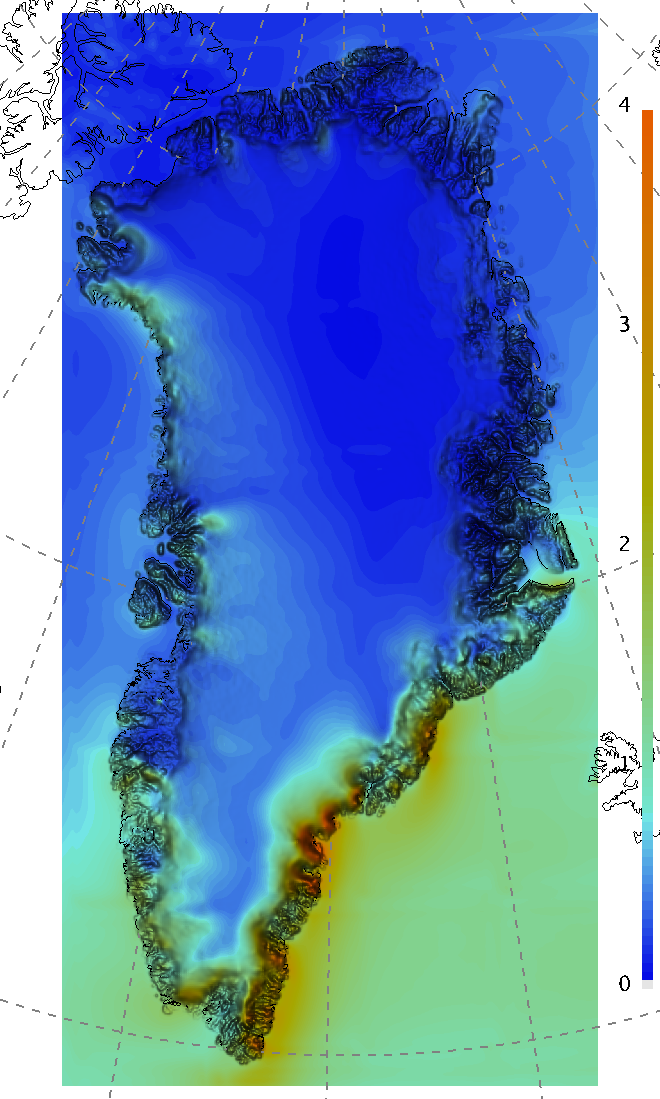
\includegraphics[width=2.5in,keepaspectratio=true]{sr-greenland-prcp}}
\caption{The input present-day ice thickness (left; m) and present-day precipitation (right; m $\text{a}^{-1}$ ice equivalent) for SeaRISE-Greenland.  Figures produced with IDV}
\label{fig:sr-input1}
\end{figure}

\begin{figure}[ht]
\centering
\mbox{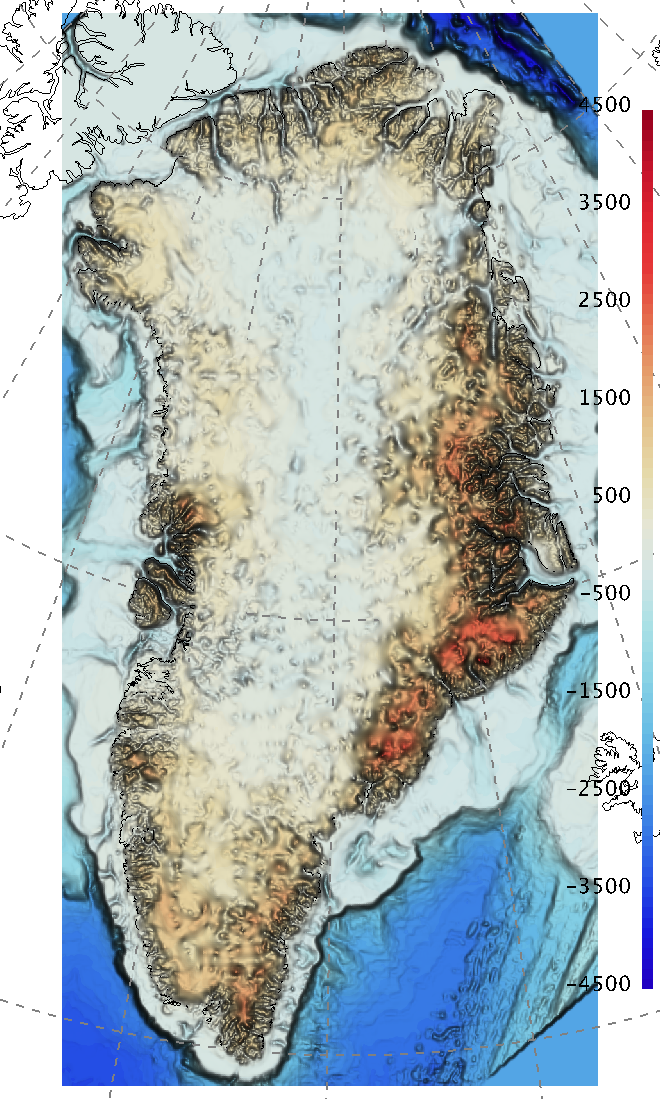
\includegraphics[width=2.5in,keepaspectratio=true]{sr-greenland-topg}
 \qquad\quad 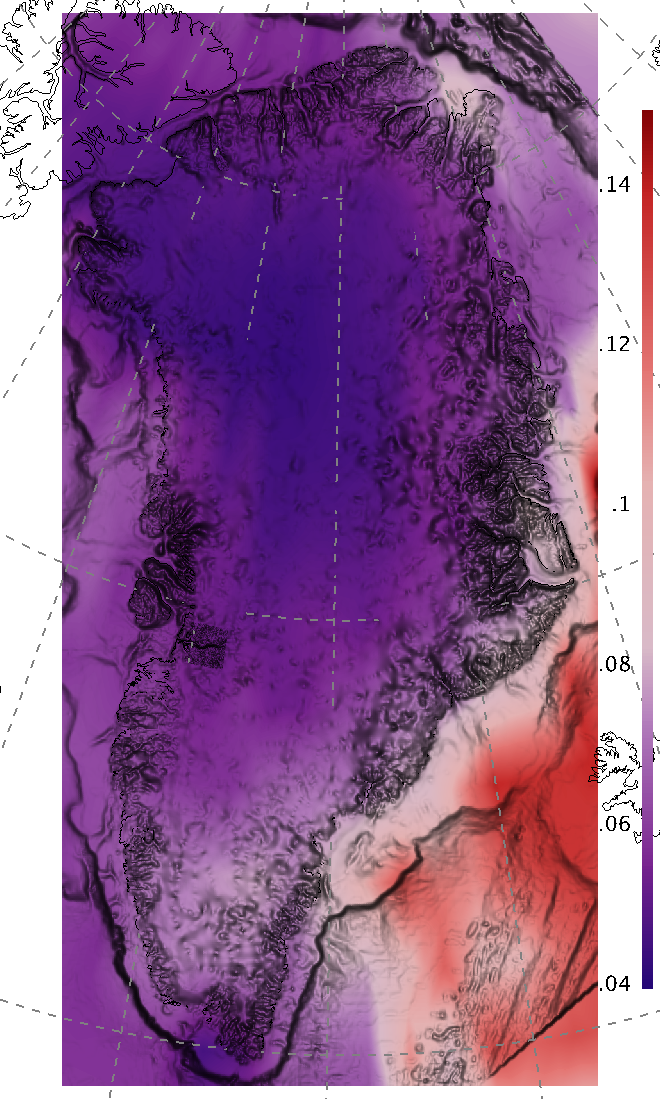
\includegraphics[width=2.5in,keepaspectratio=true]{sr-greenland-bheatflx}}
\caption{The input bedrock elevation (left; m) and geothermal flux (right; W $\text{m}^{-2}$) for SeaRISE-Greenland.  Figures produced with IDV}
\label{fig:sr-input2}
\end{figure}


\subsection{Run PISM}

We are ready to run PISM, but, perhaps even more than many unix programs, PISM allows \emph{a lot} of command-line options.  In fact, because it is an ice flow simulation program designed to handle many different ice sheets, shelves, and glaciers, the list of user-configurable flags and parameters is quite long.\footnote{We believe this is a feature not a bug.}  For a complete list of configuration flags and parameters see
\begin{center}
\url{http://www.pism-docs.org/dev/doxy/html/config.html}
\end{center}
Therefore it is wise to build a \emph{script} to run PISM with the correct options. 

Also, as explained in the rest of this \emph{User's Manual}, modeling ice sheets requires the integration of paleo-climatic and long-time-scale information into the model state, so our script is called ``\verb|spinup.sh|''.  The spin-up stage is the one which generally requires the most processor-hours, compared to a ``forecast'' stage.

To see what the SeaRISE-Greenland PISM run involves, do this:

\verb|$ PISM_DO=echo|

\verb|$ ./spinup.sh|

\noindent Setting the environment variable \verb|PISM_DO| in this way tells \verb|spinup.sh| just to print out the commands it is about to run, not do them.

Note that ``\verb|mpiexec -n 2 pismr|'' appears in the echo-ed PISM runs from \verb|spinup.sh|.  This means that the PISM executable \verb|pismr| is run in parallel on two processes (e.g.~cores on a smaller machine).  Note ``\verb|pismr|'' stands for the standard ``run'' mode of PISM, in contrast to more specific modes as described later.  Also, for the rest of this example, we assume you have a workstation with 8 cores, which is typical of 2010 resources.

The script \verb|spinup.sh| starts by ``bootstrapping.''  This means the creation, by heuristics and simplified models, of the kind of full initial conditions needed for the evolving, time-dependent model.  Specifically, the first 100 model year run with 8 processes will look like
\begin{verbatim}
mpiexec -n 8 pismr -ocean_kill -eta -skip 2 -boot_from pism_Greenland_5km_v0.93.nc \
  -Mx 76 -My 141 -Lz 4000 -Lbz 2000 -Mz 41 -Mbz 16 \
  -atmosphere searise_greenland -surface pdd -pdd_fausto \
  -y 100 -o g20km_pre100.nc
\end{verbatim}
The options describe a $76\times 141$ point grid in the horizontal, which is a 20 km grid.  There are also important choices about the vertical extent and resolution of the computational domain; more on those later.

Instead of typing-in the above PISM command with all its options, get the run going by

\verb|$ export PISM_DO=|

\verb|$ ./spinup.sh 8 >> out.spin20km &|

\noindent PISM will show what it is doing in the text (ASCII) file \verb|out.spin20km| while it runs in the background.  Using \verb|less| is good for watching a growing text file.  It will fairly quickly---within a minute---produce a very-early flow result in \verb|g20km_pre100.nc|.  Also \verb|g20km_climate-500a.nc| shows a movie of the simulated Greenland ice-sheet-model-inputs ``climate'', from 1500 to today, an important result to look at early because surface mass balance is (and must) be simulated for this kind of spinup.

The total run time for the complete 20km spinup, which models 125,000 model years with ``full physics'' of the SIA+SSA hybrid type (section \ref{sect:dynamics}) uses about 80 processor-hours.  

FIXME:  This run should take about one minute of real time. Next we generate a more credible enthalpy field. One way to do this is to have the enthalpy field and velocity field co-evolve according to the thermomechanical flow model while holding the upper ice surface stationary.  This is a continuation of ``bootstrapping''.  The effect is to create an enthalpy field which is approximately stationary with respect to advection and conduction.\footnote{The resulting enthalpy field is not a fully physical enthalpy field, however, because it comes from a steadiness assumption about the geometry of the ice sheet.  Said another way, it is a enthalpy field in equilibrium with a velocity field for which the surface kinematical equation \cite{Fowler} is \emph{not} satisfied.}  We create this enthalpy field by running for 50000 years\footnote{A longer run might be desirabe, but here we only wish to have a reasonable starting field. More about how to determine the length of a no-mass run can be found in...} with non-evolving surface.  The option \verb|-no_mass| turns off the map-plane mass continuity scheme, and thus any evolution of the surface.
\begin{verbatim}
$ mpiexec -n 4 pismr -ocean_kill -skip 2 -i g20km_pre100.nc \
  -atmosphere searise_greenland -surface pdd -pdd_fausto -no_mass -y 50000 \ 
  -extra_file ex_g20km_steady.nc -extra_vars enthalpybase,temppabase \ 
  -extra_times 0:250:50000 -o g20km_steady.nc
\end{verbatim} This takes about 1 hour (4 processor hours). Before we proceed with the actual paleo-climate forcing, we add another short smoothing run:
\begin{verbatim}
$ mpiexec -n 4 /pismr -ocean_kill -skip 2 -i g20km_steady.nc \
  -atmosphere searise_greenland -surface pdd -pdd_fausto \
  -y 100 -o g20km_SIA.nc
\end{verbatim}



%%%%  OLD




\subsection{Handling NetCDF files}\label{subsect:nctoolsintro}  At a superficial level, \verb|pismr| is just a program which takes one or more NetCDF files as input, does some computation, and produces one or more NetCDF files as output.  The user is in charge of creating NetCDF input files containing data on ice sheets worth modeling\footnote{See the section \ref{sec:bootstrapping-format} and table \ref{tab:modelhierarchy} for a hint about data necessary for modeling.}, and extracting some meaning from the NetCDF output files.

The most basic tools for converting NetCDF files to and from a standard text representation are called \verb|ncdump| and \verb|ncgen|.  A glance at Unix \verb|man| pages for these tools might be wise at this time.

As suggested earlier, we regularly use \verb|ncview| to look at NetCDF files.  The NetCDF tools most frequently used by the PISM developers are shown in Table \ref{tab:NetCDFview}.  This website gives additional NetCDF-related tools:

\centerline{ \href{http://www.unidata.ucar.edu/software/netcdf/docs/software.html}{\t{www.unidata.ucar.edu/software/netcdf/docs/software.html}} } 

\newcommand{\netcdftool}[1]{#1\index{NetCDF!tools!#1}}
\begin{table}[ht]
\centering
\caption{Some tools for viewing and modifying NetCDF files.}\label{tab:NetCDFview} 
\small
\begin{tabular}{@{}llll}\hline
\textbf{Tool} & \textbf{Site} & \textbf{Function}\\ \hline
\netcdftool{\texttt{ncdump}} & \emph{included with any NetCDF distribution} & dump binary NetCDF as \texttt{.cdl} (text) file \\
\netcdftool{\texttt{ncgen}} & \emph{included with any NetCDF distribution} & convert \texttt{.cdl} file to binary NetCDF \\
\netcdftool{\texttt{ncview}} & \href{http://meteora.ucsd.edu/~pierce/ncview_home_page.html}{\texttt{meteora.ucsd.edu/$\sim$pierce}} & quick graphical view \\
\netcdftool{IDV} & \href{http://www.unidata.ucar.edu/software/idv/}{\t{www.unidata.ucar.edu/software/idv/}} & more complete visualization \\
\netcdftool{Paraview} & \href{http://www.paraview.org}{\t{www.paraview.org}} & powerful open-source parallel visualization \\
\netcdftool{NCL} &  \href{http://www.ncl.ucar.edu}{\t{www.ncl.ucar.edu}} & NCAR Command Language, open-source\\
\netcdftool{PyNGL} &  \href{http://www.pyngl.ucar.edu}{\t{www.pyngl.ucar.edu}} & Python version of NCL, open-source\\
\netcdftool{VisIt} & \href{http://visit.llnl.gov}{\t{visit.llnl.gov}} & advanced parallel visualization \\
\netcdftool{NCO}\index{NCO (NetCDF Operators)} & \href{http://nco.sourceforge.net/}{\t{nco.sourceforge.net/}} & ``NetCDF Operators'': manipulations \\
\quad  & & \quad at command line
\end{tabular}
\normalsize
\end{table}


%%% Local Variables: 
%%% mode: latex
%%% TeX-master: "manual"
%%% End: 

